\chapter{Strings-and-winds development studies}\label{app:phase2dev}
This appendix collects the development studies of the strings-and-winds
setting in full. Each of them keeps a short summary in
Chapter~\ref{ch:phase2}. All of the evidence reported here comes from the
development set under the protocol of \S\ref{sec:hygiene}, and none of the
hypotheses evaluated on the held-out test set depended on any of it. The
appendix opens with the meaning of the six channels in musical terms, then
reports the drift study of within-note variation, the exploratory
tonal-metric test on intonation, and the comparison of three priors at
track scale.

\section{The channels in musical terms}\label{app:glossary}
Before the estimation machinery, it helps to say what these quantities mean
to a listener. \textbf{Intonation} $c_i$ is whether a note is played sharp
or flat, and by how much. It is the deviation of the held pitch centre of
the note from the position that equal temperament assigns to the written
note, measured in cents, one hundred cents to a semitone, with positive
values meaning sharp. The centre is the centre of the pitch curve with the
vibrato oscillation removed, and it is not, by design, the average of the
curve, for the reason given in the drift study below. \textbf{Vibrato} is
the intentional periodic oscillation of pitch around that centre which
singers, string players and wind players add to sustained notes
\cite{seashore1936}. Three numbers describe it per note. The rate
$f_i^{\mathrm{vib}}$ is the number of oscillations per second, typically
five to eight, with a mean of $6.0$\,Hz \cite{prame1994}. The extent
$\gamma_i$ is how far the pitch swings from the centre at its peak, in
cents: tens of cents on the strings and winds studied here, and
$\approx 71$ cents on average in professional singing \cite{prame1997}. The
onset delay $d_i^{\mathrm{vib}}$ is how long after the note begins the
oscillation starts, since performers often begin a note straight and let
the vibrato grow. \textbf{Loudness} $\ell_i$ is how strongly the note
sounds, read from the energy of the audio through \eqref{eq:loudness} and
taken relative to the level of the recording itself.

None of these values is annotated by hand. Every one of them is estimated
from the recording: a pitch tracker supplies the pitch curve of the note,
and the per-note fit turns that curve into these numbers, each with its own
uncertainty, which is exactly why the observation noise of
\eqref{eq:phase2-noise} becomes substantial on tracked audio. The human
annotations of the corpus supply only the note spans, that is, the onsets,
the durations and the written pitches. The annotated pitch curves of the
corpus, the reference curves, serve to calibrate the tracker and are never
used as channel values.

\section{The drift study of within-note variation}\label{app:drift}
Equations \eqref{eq:loudness} to \eqref{eq:vibrato} hold every parameter
fixed within the note, so the channels are time-averages, and it is fair to
ask what the averaging discards. The study that answers this is simple.
Every vibrato-identifiable development note that both pitch curves can
measure ($n = 5{,}145$) is refitted with the vibrato model of
\eqref{eq:vibrato} plus one added ingredient, a linear drift of the centre,
$c + s\,(t - \bar t)$ under the vibrato, and the fit is run twice per note,
independently on the tracked curve and on the reference curve. The
two-curve design is the control: a slope that appears in one curve only
would be measurement noise, whereas a slope that two independent
measurements agree on is the player. Loudness receives the same check
through the four chunk levels of \eqref{eq:loudness}.
Table~\ref{tab:drift-study} collects the numbers and
Figure~\ref{fig:drift-study} shows the argument.

\begin{table}[t]\centering
\caption{Within-note time variation on the development set. Intonation
slopes are fitted independently on the tracked and on the reference
curves, loudness slopes on the four chunk levels of \eqref{eq:loudness}.
The last row is the across-note test of whether the discarded structure is
one that a graph over notes could use.}
\label{tab:drift-study}
\footnotesize
\begin{tabular}{@{}lcc@{}}
\toprule
 & intonation drift & loudness slope \\
\midrule
notes with a significant slope & $65.5\%$ / $67.1\%$ (tracker / truth) & $41.3\%$ \\
the two curves agree on direction & $97\%$ (rank corr.\ $0.91$) & --- \\
typical size (median) & $10.5$ cents per note (q90 $32$) & $1.4\times$ the across-note sd of $\ell$ \\
share falling (decay envelope) & --- & $65\%$ (brass $81\%$, strings $57\%$) \\
across-note lag-1 correlation & $+0.03$ & $+0.06$ \\
\quad (reference: timing $\tau$) & \multicolumn{2}{c}{$+0.59$} \\
\bottomrule
\end{tabular}
\end{table}

\begin{figure}[t]
  \centering
  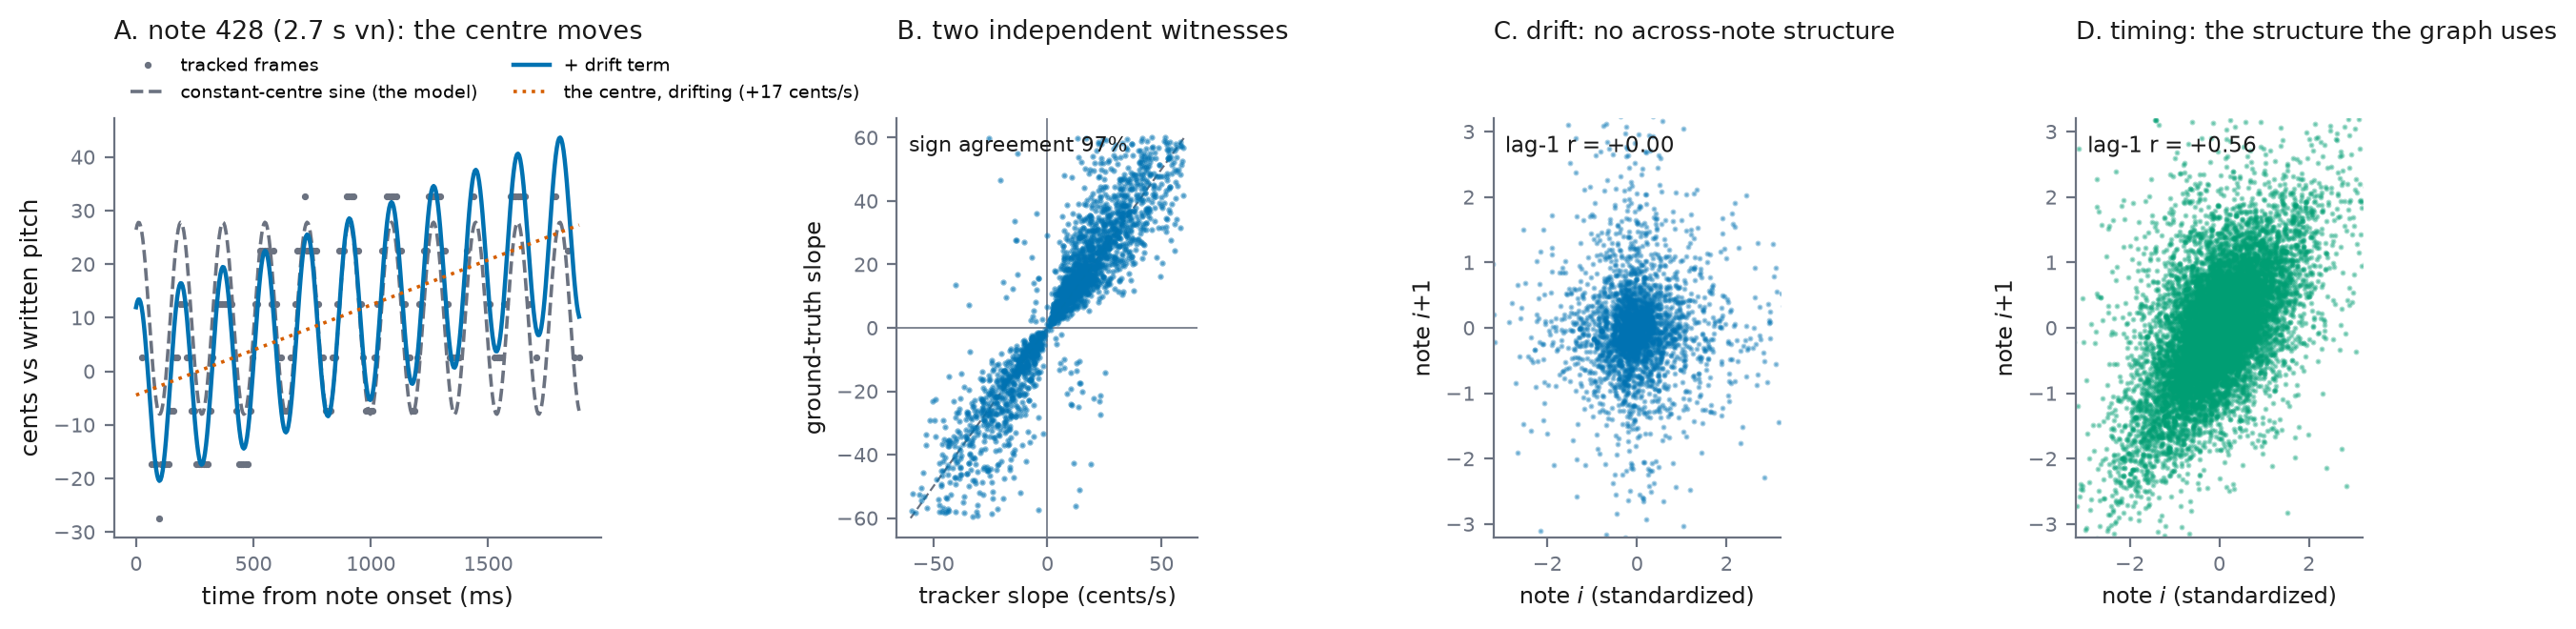
\includegraphics[width=\linewidth]{figures/drift_study_dev.png}
  \caption{The drift study in four panels, on the development set.
  Panel A: a $2.7$-second violin note, where the constant-centre sine
  (dashed) holds the centre flat and the drift term shows the centre
  climbing at $+17$ cents/s under the vibrato. Panel B: on the notes where
  both curves fit a significant slope, the slope from the tracked curve
  against the slope from the reference curve, the two agreeing on direction
  $97\%$ of the time. Panel C: the drift slope of note $i$ against that of
  note $i{+}1$, standardized per track and pooled, with no across-note
  structure. Panel D: the same plot for the timing residual $\tau$, the
  across-note correlation that the graph prior uses. Panels A and B show
  the within-note structure that the sine model discards, and panels C and
  D the across-note structure on which the graph operates.}
  \label{fig:drift-study}
\end{figure}

The findings follow in the order of their importance. The drift is music
rather than tracker noise: about two thirds of the notes carry a
significant slope in each curve independently, and the two curves agree on
its direction $97\%$ of the time (panel B of Fig.~\ref{fig:drift-study}).
The drift is also large relative to the reported precision. The median note
drifts by $10.5$ cents, an order of magnitude above the median reported
standard error of $0.9$ cents on the intonation channel, so $c$ is a
precise estimate of the \emph{average} intonation of the note rather than
of a constant (panel A of Fig.~\ref{fig:drift-study}). Loudness moves even
more, although the falling shares in Table~\ref{tab:drift-study} indicate
that most of its movement is decay envelope rather than expressive shaping.
The discarded structure, finally, is white with respect to the graph. The
within-note slopes carry essentially no correlation from one note to the
next, where timing, the channel the graph demonstrably helps, carries
$+0.59$ (panels C and D of Fig.~\ref{fig:drift-study}).

Three consequences keep the per-note resolution defensible rather than
refuted. The mismatch is priced into the noise model, since the per-note
variances of \eqref{eq:phase2-noise} are residual-based, so a drifting note
reports itself as more uncertain, which is why calibration held on the
held-out test set. The reference targets pass through the same
parameterization, so the contrasts between the graph model and the no-graph
model compare like with like. And a within-note slope channel is precisely
the kind of channel that the graph prior could not help, so the per-note
resolution is empirically the right level for this model. The discarded
structure itself belongs to the frame-level likelihood of the waveform
setting, whose amplitude envelope $A_i(t)$ and pitch-curve model are built
to carry it. Slope channels remain candidates for a later evaluation under
the $d^{\mathrm{vib}}$ template, included as output with no hypothesis
attached to them.

\section{The tonal-metric exploratory test on intonation}\label{app:tonal}
The hypothesis of \S\ref{sec:phase2-delta}, that a circle-of-fifths metric
would improve the intonation channel, was fixed before the numbers were
seen, and the test was designated exploratory in the pre-specified design.
On the development set, replacing the semitone metric by the
circle-of-fifths metric improves held-out intonation on both axes. The
paired difference, tonal minus plain under the given variances, is $-0.21$
cents in RMSE with interval $[-0.34, -0.09]$ and $-0.05$ in NLL with
interval $[-0.07, -0.03]$, both intervals excluding zero. The replacement
also re-imposes the familiar penalty on timing, an NLL difference of
$+0.03$ against the tonal metric with an interval excluding zero. The
vibrato-rate channel picks up a small recovery gain of $-0.027$, with an
interval excluding zero, and the remaining channels are indifferent
(Fig.~\ref{fig:tonal-intonation}). On the held-out test set, under the
re-use described in \S\ref{sec:phase2-reuse}, the recovery gain was
reproduced, at $-0.312$ cents with interval $[-0.599, -0.081]$, whereas the
calibration difference, $-0.023$ with interval $[-0.049, +0.001]$, was not.
The tonal metric therefore keeps its exploratory status.

\figph{tonal_intonation_dev.png}{1.0}{The exploratory circle-of-fifths
contrast on intonation on the development set: paired RMSE differences per
track-and-seed combination, tonal minus plain graph, under the given
variances. The mean is $-0.21$ cents with interval $[-0.34, -0.09]$,
$61\%$ of the pairs improve, and the full spread is shown. On the held-out
test set (\S\ref{sec:phase2-reuse}) the recovery gain was reproduced at
$-0.31$ cents with an interval excluding zero, and the calibration
difference of $-0.023$ had an interval reaching
zero.\label{fig:tonal-intonation}}

\section{Three priors at track scale}
\label{app:trackscale}
The waveform studies of Chapter~\ref{ch:phase3} found, on chains of three
to ten notes, that the score prior transfers only the common offset of the
context. The same question can be asked at whole-track scale on the tracked
six-channel bundle of this chapter. There, the development evaluation
already holds out $30\%$ of the notes per track, and both the graph model
and the no-graph ablation carry a per-piece bias column, so every contrast
is a contrast beyond the common offset. Two further priors were added to
that evaluation on the development set, with their hypotheses fixed in
advance, over $78$ tracks and $153$ track-and-seed combinations, under the
given variances and with paired differences per combination. The first is
a time-only chain, the same GP with the score graph replaced by unit-weight
edges between consecutive notes. The second is a time-only Gaussian graph,
the score graph with its pitch term removed and its two-beat time window
kept.

\begin{table}[t]\centering
\caption{Three priors at track scale on the strings-and-winds bundle, on
the development set. Paired differences per track-and-seed combination
against estimator targets, with $95\%$ bootstrap intervals. Negative
favours the first-named arm, and $*$ marks an interval excluding zero.
Intonation is in cents, vibrato extent and rate on the log scale.}
\label{tab:trackscale}
\footnotesize
\begin{tabular}{@{}lccc@{}}
\toprule
channel & score graph $-$ chain & score graph $-$ time-Gaussian & time-Gaussian $-$ chain \\
\midrule
intonation $c$, RMSE & $-0.50$ $[-0.67,-0.34]*$ & $-0.02$ $[-0.10,+0.06]$ & $-0.48$ $[-0.65,-0.32]*$ \\
intonation $c$, NLL & $-0.037*$ & $+0.006$ & $-0.043*$ \\
vibrato extent, RMSE & $-0.22*$ & $+0.04*$ & $-0.27*$ \\
vibrato rate, RMSE & $-0.21*$ & $+0.03*$ & $-0.24*$ \\
loudness, RMSE & $-0.007*$ & $-0.007*$ & $-0.000$ \\
timing, RMSE & $-0.001$ & $+0.000$ & $-0.002$ \\
\bottomrule
\end{tabular}
\end{table}

The result is two-sided in the same way as the waveform spans, but with the
statistical power that the chains lacked. The score graph is better than
the time-only chain on intonation, vibrato extent, vibrato rate and
loudness, with intervals excluding zero (Table~\ref{tab:trackscale}, first
column), and the chain itself is not reliably better than no structure,
since its NLL is worse on loudness and vibrato onset. The score graph shows
no measurable difference from the time-only Gaussian graph on intonation
($-0.02$ cents, with an interval covering zero) and is slightly worse on
the two vibrato channels. The time-only Gaussian graph against the chain
reproduces the margins of the score graph, and against no structure it
reproduces the intonation gain of the score graph that the held-out
evaluation established ($-0.88$ against $-0.90$). The value of the graph at
track scale is therefore temporal smoothing over a window of about two
beats. The pitch-proximity coupling that makes it a \emph{score} graph adds
nothing measurable here, as it added nothing at chain and phrase scale from
the waveform.

The piano counterpart gives the same answer. The piano model of
Chapter~\ref{ch:results} with the pitch term removed from its graph, the
two-beat window kept, which on polyphonic piano links the notes of a chord
at full weight, was paired per piece against the full model on the
development set, over $30$ pieces and $4$ seeds. The pooled RMSE difference
is $-0.008$ with interval $[-0.016, -0.001]$ and the NLL difference is
$-0.019$ with interval $[-0.030, -0.008]$, a small improvement whose
intervals exclude zero, carried by articulation. The total value of the
graph on that set is $+0.017$ RMSE, so the pitch-less graph is worth about
half again as much as the score graph. On both corpora, then, the structure
that does the work is smoothness in score time over about two beats,
including the vertical coupling of simultaneous notes, and pitch proximity
adds nothing and costs a little. This attributes the graph value
established on the held-out test set without retracting it, since the
held-out comparisons are of the full model against its alternatives, and a
pitch-less graph as the default would change a reported protocol and
require its own pre-specified held-out evaluation.\footnote{The three
track-scale comparisons are recorded in
\texttt{results/phase2\_chain\_prior\_dev.md},
\texttt{results/phase2\_timegauss\_prior\_dev.md} and, for the piano
counterpart, \texttt{results/piano\_timegauss\_dev.md}.}
